\section{Traceability Support}\label{sec:traceability}
This section describes tool support for traceability along the \into tool chain.
%
%
%
\subsection{Overview}
Traceability support is divided into two steps: sending data from the tools to the Neo4J traceability database, and retrieving information from the database. In the following we first describe how information is sent to the database and then how it is retrieved.

It shall be noted that the traceability features of INTO-CPS require Git\footnote{\url{https://git-scm.com/}} to be installed. Furthermore, the project folder must be under Git version control.
%
\subsection{INTO-CPS Application}
Information is stored in the traceability database via the traceability daemon.  The traceability daemon is integrated in the \intoapp{} and it starts automatically when the Application is started. Only Neo4J has to be downloaded, which can be done through the Download Manager. When downloaded, Neo4J must be extracted by hand into the folder \texttt{<user\_home>/into-cps-projects/install} (the archive file is located at \texttt{<user\_home>/into-cps-projects/install\_downloads} after download.) Note that Neo4J is a singleton, so ensure all other instances of Neo4J are down before starting the \intoapp. 

Please note: the daemon only runs while the \intoapp{} is running. Therefore, to record traceability data while using any of the other tools, the \intoapp{} must be running.

Treaceability information is captured by the traceability daemon and stored in a Neo4J database. The database is project-specific and is deployed on project change within the \intoapp. When running, Neo4J is accessible at \url{http://localhost:7474}. Here one can view the current traceability graph.  Username and password of the databases are always:

username = intoCPSApp\\
password = KLHJiK8k2378HKsg823jKKLJ89sjklJHBNf8j8JH7FxE\\

To view the raw data from the database, right-click on \textit{Traceability} in the \intoapp{} project browser and select \textit{View Traceability Graph} (see Figure \ref{fig:app_trace}). Select the database symbol and click under \textit{Relationship types} click on \textit{Trace}. This shows the graph database. By default, the view is limited to 25 entries. To change this, edit the line \texttt{MATCH p=()-[r:Trace]->() RETURN p LIMIT 25} and set the limit to a different value. When starting the \intoapp{}, Neo4J needs to be started as well. Sometimes this is very slow and the startup operation is aborted. To force the Neo4J database to start, repeat the \textit{View Traceability Graph} action until the Neo4J view shows, as illustrated in Figure \ref{fig:app_trace}. Alternatively, start the INTO-CPS Application from the command line to monitor the status of the Neo4J database.
%
%
%
\begin{figure}[htbp]
	\centering
		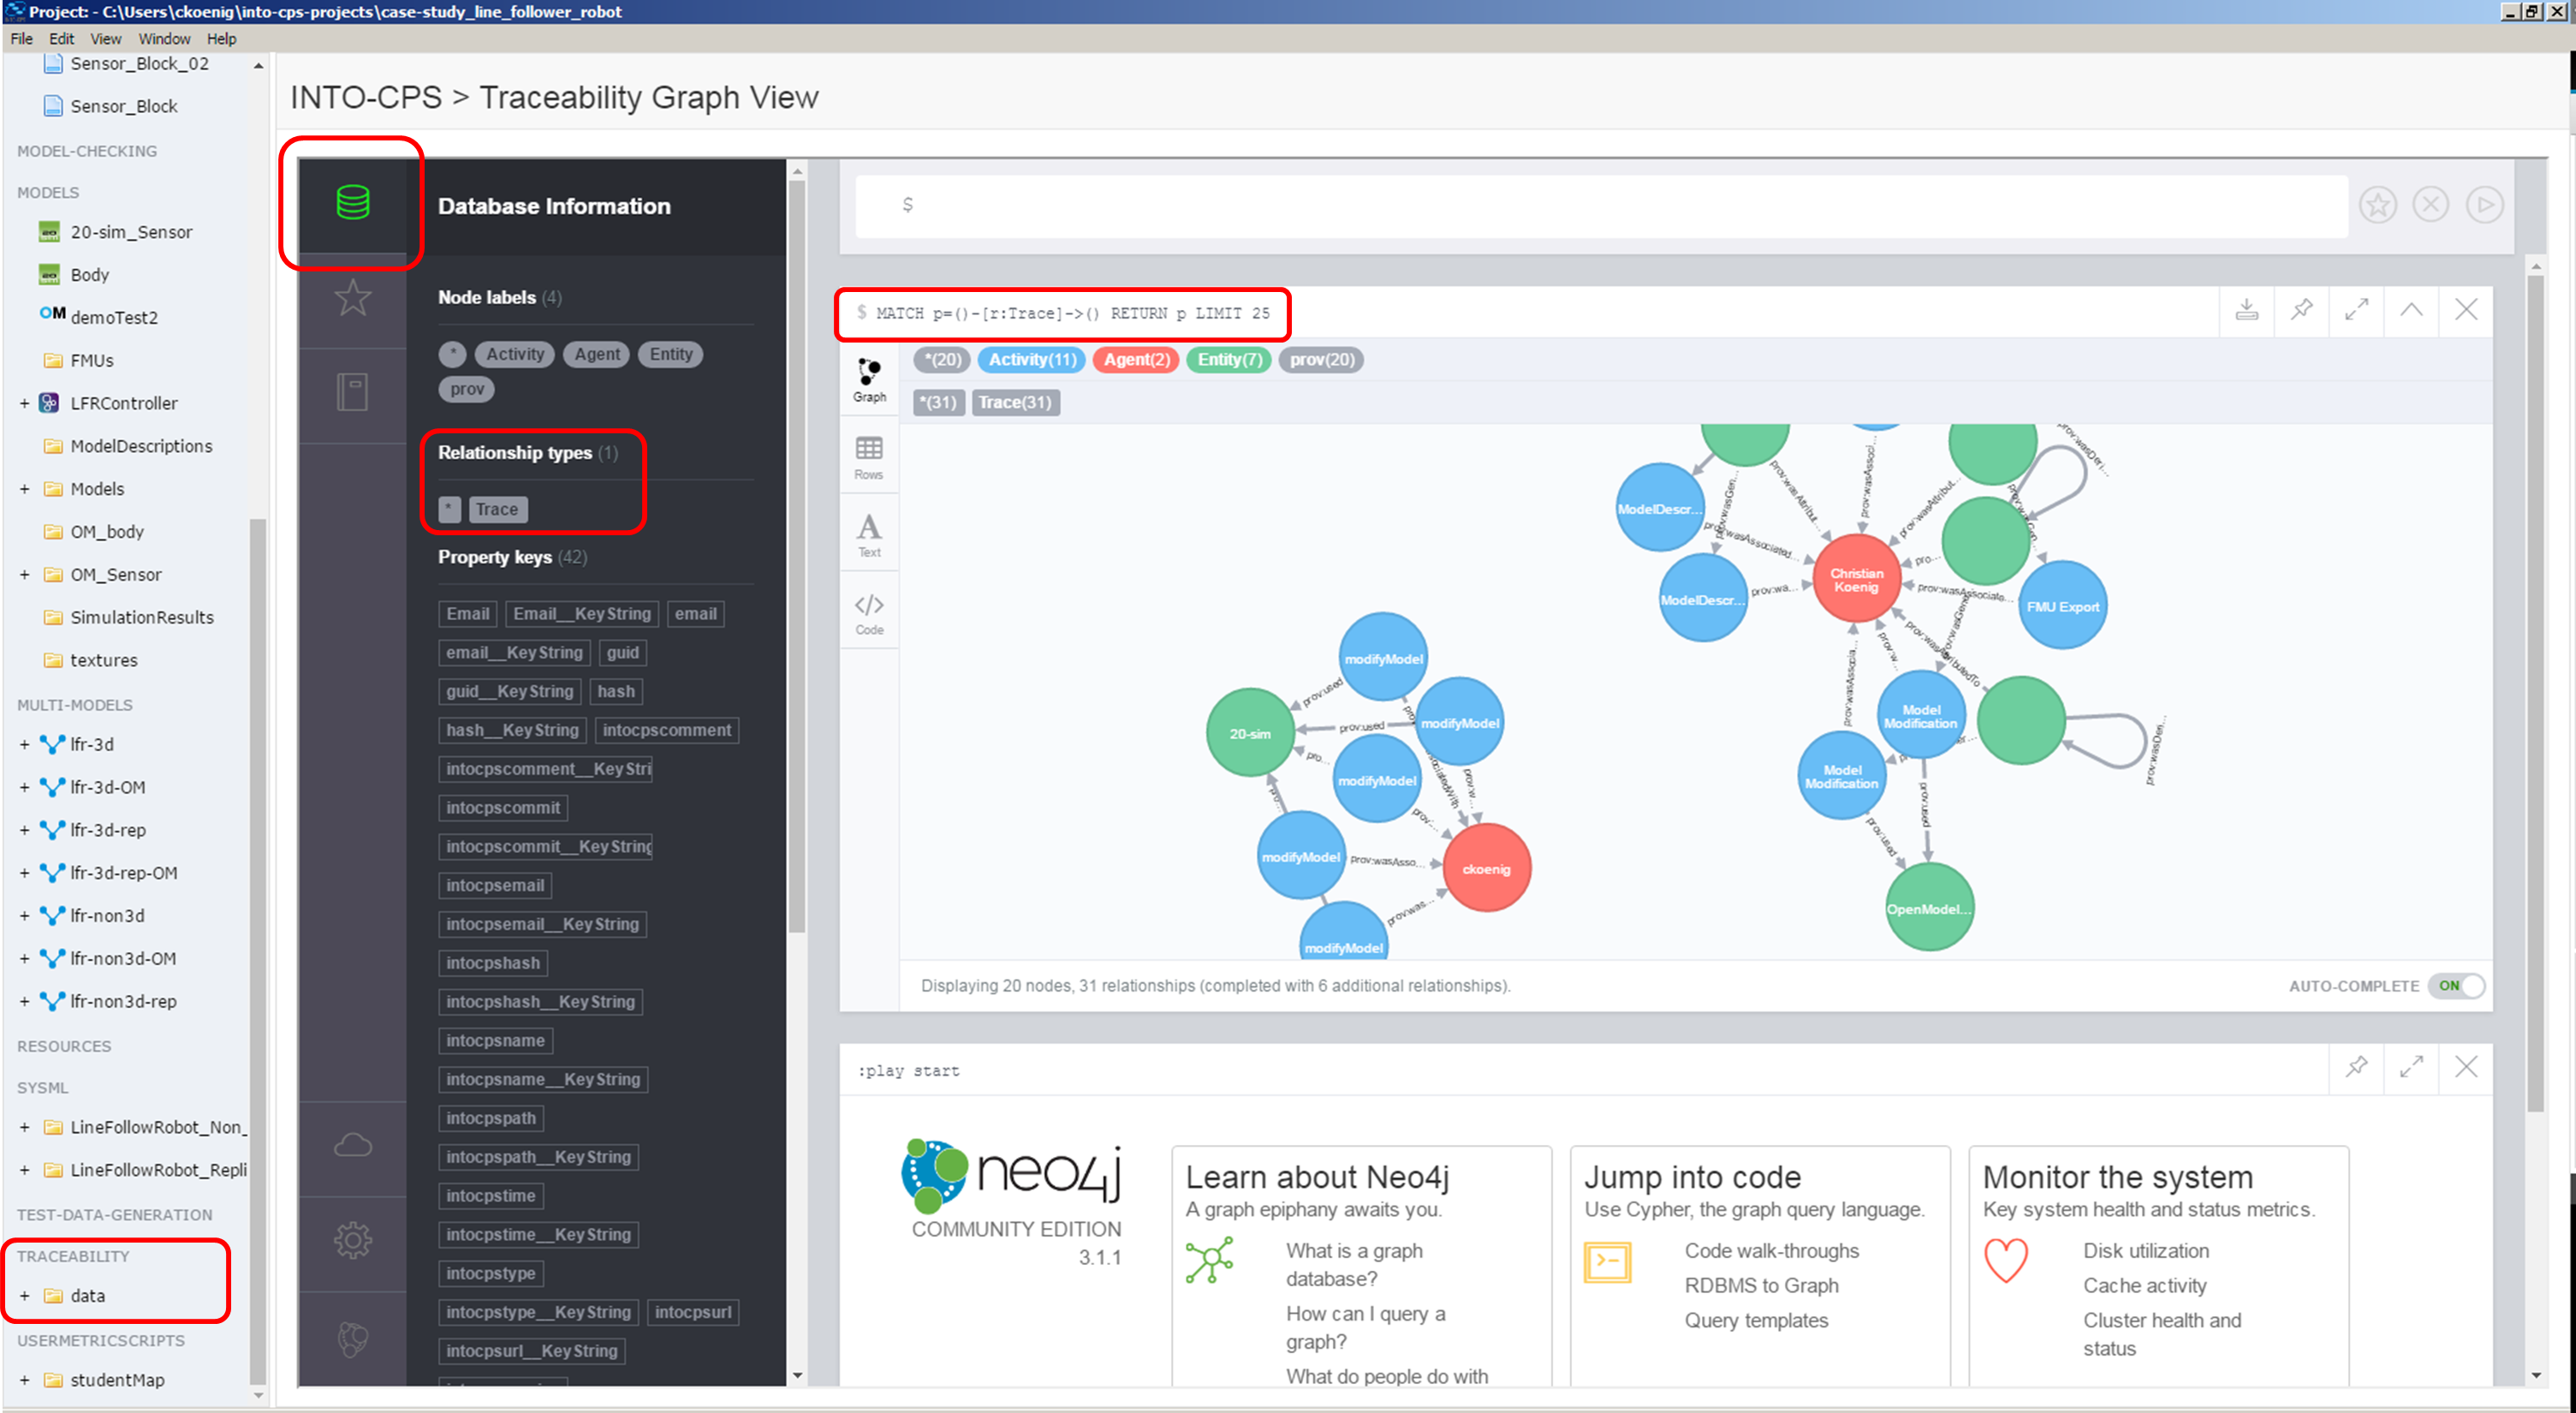
\includegraphics[width=1.00\textwidth]{figures/app_traceability01.png}
	\caption{Current view of traceability in the \intoapp.}
	\label{fig:app_trace}
\end{figure}
%
%
%
Please note: this view of traceability relationships is not meant for end users, but rather for developers.
%
%
%
\subsection{Modelio}
The latest Modelio module can be downloaded here:  \url{http://forge.modelio.org/projects/intocps-modelio34/files}.  Note that currently the INTO-CPS module is only compatible with Modelio 3.4.
%
Modelio currently (INTO-CPS module 1.3.15) supports traceability for the following modelling activities:
%
%
%
\begin{itemize}
\item Model creation
\item Model modification
\item Model Description export
\item Configuration export
\item Requirements creation
\end{itemize}
%
To install the module go to \emph{Configuration \textrightarrow{} Modules}, select \emph{INTO-CPS} and set the parameters for:
\begin{itemize}
 \item The daemon connection, \emph{i.\@e.\@} the daemon IP address and its connection port (7474). By default these values are, respectively, 127.0.0.1 and 8083
\item The Git user identification, \emph{i.\@e.\@} its Git ID, the related e-mail address and the path to the local Git repository (\emph{i.\@e.\@} the path to the location of the \texttt{.git} folder).
\end{itemize}
%
%
%
\begin{figure}[htbp]
\centering
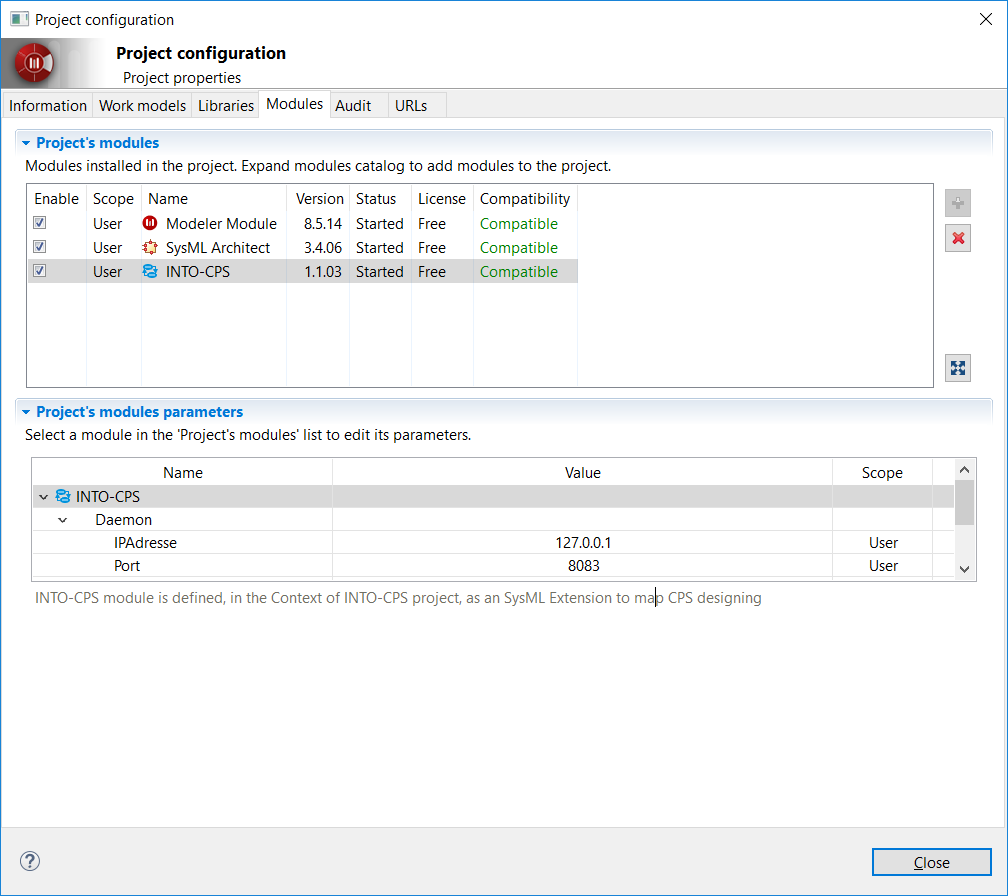
\includegraphics[width=0.8\textwidth]{figures/Modelio_moduleConfiguration}
\caption{Configuration of traceability features in Modelio.}
\label{fig:modelio_trace_config}
\end{figure}
%
The traceability information is sent automatically to the daemon, either right after performing a traced action (Model Description Export and Configuration Export) or after closing the project.

Regarding requirements tracing, currently only the relations \textit{Satisfy} and \textit{Verify} are supported for traceability, as shown in Figure \ref{fig:modelio_trace_req}.
%
\begin{figure}[htbp]
\centering
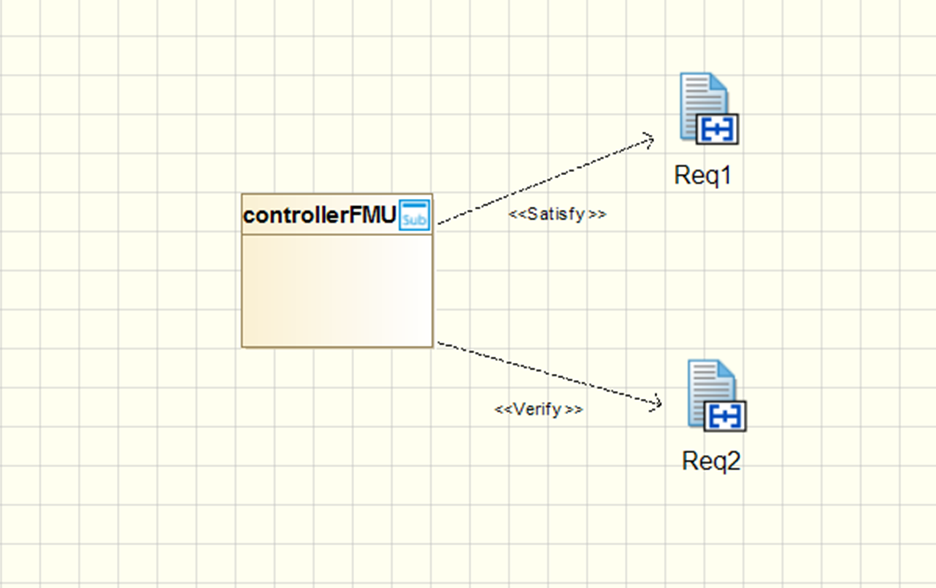
\includegraphics[width=0.7\textwidth]{figures/modelio_trace_req}
\caption{Requirements related to a SysML Block in Modelio.}
\label{fig:modelio_trace_req}
\end{figure}
%
Hint: To push an older model (\emph{i.\@e.\@}, one made before the deployment of the traceabilty feature) to the traceability database, you can use the following Jython script inside the Modelio \emph{Script} tab as depicted in Figure \ref{fig:modelio_push_script}.
%
\begin{lstlisting}
peerModule = Modelio.getInstance().getModuleService().getPeerModule(IINTOCPSPeerModule.MODULE_NAME);
peerModule.pushModel();
\end{lstlisting}
%
\begin{figure}[htbp]
\centering
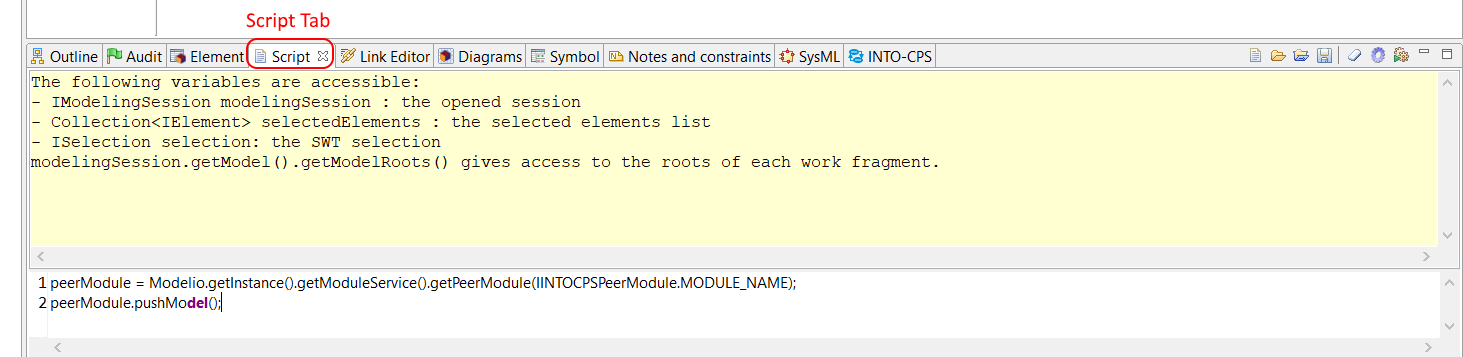
\includegraphics[width=0.9\textwidth]{figures/modelio/traceability_push_script}
\caption{Pushing Jython script.}
\label{fig:modelio_push_script}
\end{figure}
%
%
%
\subsection{Overture}
The latest version of the Overture traceability driver can be found on the GitHub site\footnote{see \url{https://github.com/overturetool/intocps-tracability-driver/releases}} or in the download manager of the INTO-CPS Application.

All traces can be extracted from the traceability driver and sent to the daemon. To do so, please follow the description on the GitHub site above.
%
%
\subsection{OpenModelica}
%
The latest INTO-CPS targeted nightly builds of OpenModelica support traceability.  They can be downloaded from \url{https://build.openmodelica.org/omc/builds/windows/nightly-builds/intocps/}.  OpenModelica supports tracing the following modeling activities:
%
\begin{itemize}
	\item Model creation
  	\item Model modification
  	\item FMU export
	\item FMU import
  	\item Model description XML import
\end{itemize}
%
As a prerequisite for traceability support, Git should be installed in the system.
%
To configure traceability support, go to \emph{Tools \textrightarrow{} Options \textrightarrow{} Traceability}, select the traceability checkbox and set all the fields, the traceability daemon IP address and port (7474) (see Figure \ref{fig:OM_trace_config}). By default, the port is 8083.
%
\begin{figure}[htbp]
\centering
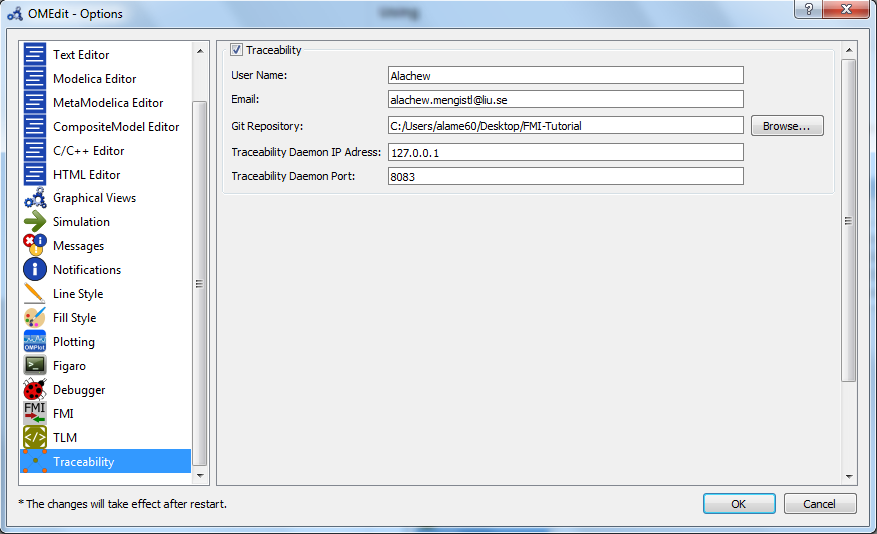
\includegraphics[width=0.7\textwidth]{figures/OM_trace01}
\caption{Traceability settings in OpenModelica.}
\label{fig:OM_trace_config}
\end{figure}
%
Then, go to \emph{Tools \textrightarrow{} Options \textrightarrow{} General} and set the working directory to which you would like to export the FMU (see Figure \ref{fig:OM_trace_config2}). 
%
\begin{figure}[htbp]
\centering
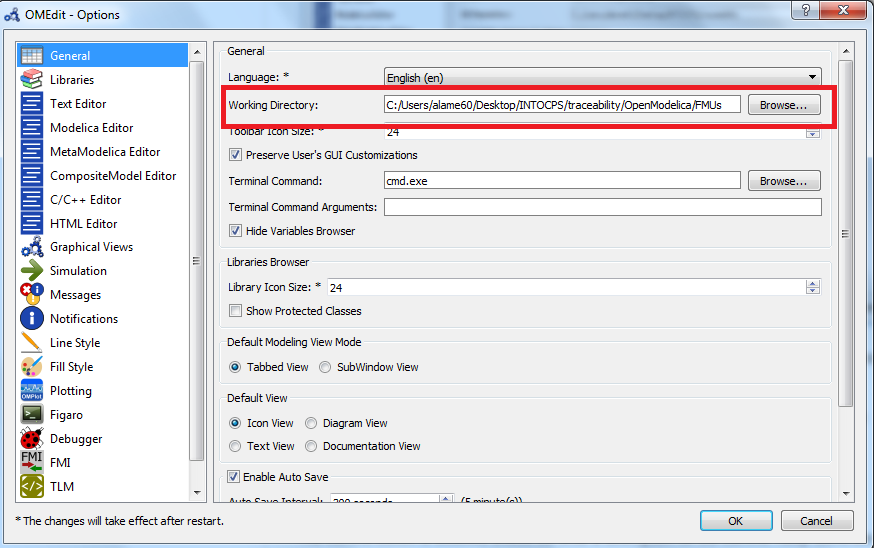
\includegraphics[width=0.7\textwidth]{figures/OM_trace02}
\caption{FMU export directory in OpenModelica.}
\label{fig:OM_trace_config2}
\end{figure}
%
Create a Modelica model via \emph{File \textrightarrow{} New Modelica Class} or load a model via \emph{File \textrightarrow{} Open Model/LibraryFile(s)}, as in Figure \ref{fig:OM_trace_config3}.
%
\begin{figure}[htbp]
\centering
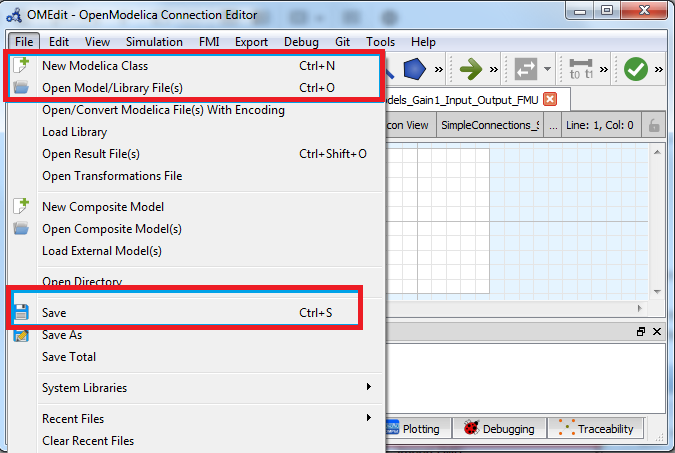
\includegraphics[width=0.7\textwidth]{figures/OM_trace03}
\caption{Create or open a Class in OpenModelica.}
\label{fig:OM_trace_config3}
\end{figure}
%
%In order to send the traceability information for the model, go to \emph{Git > Traceability > Push Traceability Information}. A dialog will appear as shown below displaying the traceability information in JSON message format. Press the \emph{Push} button and the traceability information will be stored in the Neo4J database via the traceability daemon.
%
After modification of the model/class, click the \emph{File \textrightarrow{} Save} button, press \texttt{Ctrl-s} or click the \emph{Save} button from the menu bar, as shown in Figure \ref{fig:OM_trace_config4}. A dialog as shown below in Figure \ref{fig:OM_trace_config4b} will appear to enter the commit description.
%
\begin{figure}[htbp]
\centering
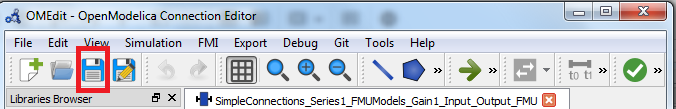
\includegraphics[width=0.7\textwidth]{figures/OM_trace04}
\caption{Save a model in OpenModelica.}
\label{fig:OM_trace_config4}
\end{figure}
%
\begin{figure}[htbp]
\centering
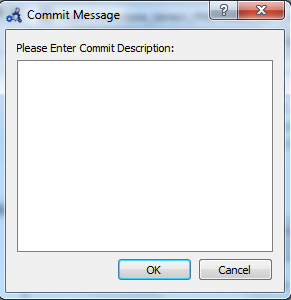
\includegraphics[width=0.5\textwidth]{figures/OM_trace04b}
\caption{The commit message in OpenModelica.}
\label{fig:OM_trace_config4b}
\end{figure}
%
To trace the export of an FMU, load the Modelica model or create a new model, then go to \emph{FMI \textrightarrow{} Export FMU} (see Figure \ref{fig:OM_trace_config6}). OpenModelica generates the FMU, commits and sends the traceability information to the daemon automatically.
%
\begin{figure}[htbp]
\centering
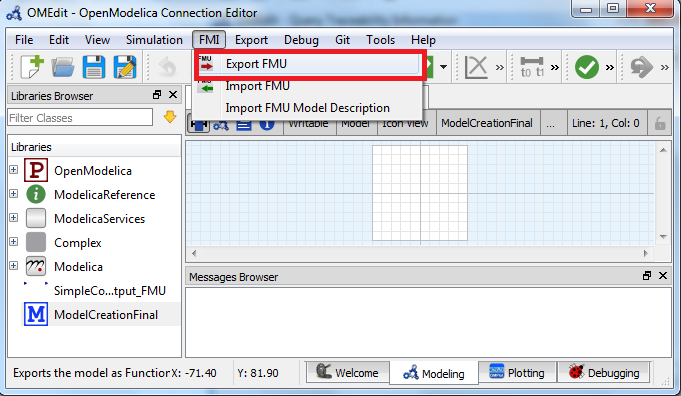
\includegraphics[width=0.7\textwidth]{figures/OM_trace06}
\caption{FMU export in OpenModelica.}
\label{fig:OM_trace_config6}
\end{figure}

To import a \texttt{modelDescription.xml} file, go to \emph{FMI \textrightarrow{} Import FMU Model Description}. A dialog as shown in Figure \ref{fig:OM_trace_config7} will appear. Select the \texttt{modelDescription.xml} file and the output directory then press \emph{OK}. The Modelica model with SysML block inputs and outputs will be generated and automatically loaded (see the left part of Figure \ref{fig:OM_trace_config7}).
%
\begin{figure}[htbp]
\centering
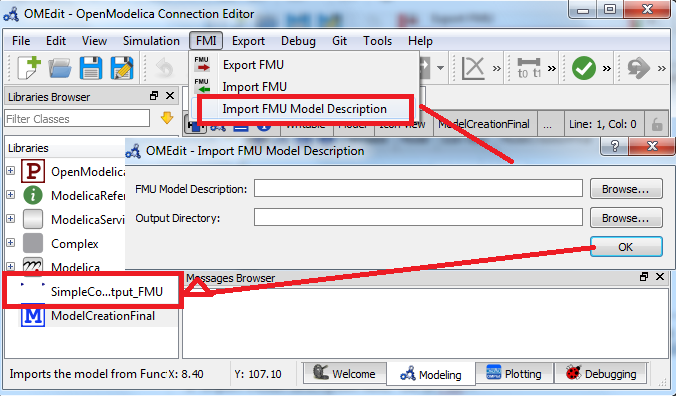
\includegraphics[width=0.7\textwidth]{figures/OM_trace07}
\caption{FMI model description import in OpenModelica.}
\label{fig:OM_trace_config7}
\end{figure}
%
To visualize the traceability graph, click the \emph{Traceability} perspective button as shown below.
%
\begin{figure}[htbp]
\centering
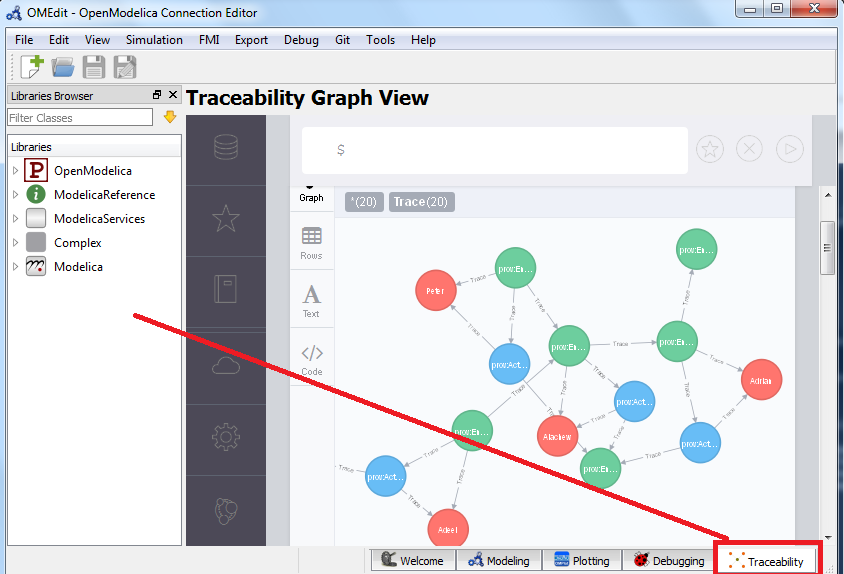
\includegraphics[width=0.7\textwidth]{figures/OM_trace08}
\caption{View traceability data in OpenModelica.}
\label{fig:OM_trace_config8}
\end{figure}
%
%some text
%
%
%
\subsection{20-sim}
To record traceability information from within 20-sim, 20-sim 4.6.3-intocps or higher is required. A version of 20-sim that supports traceability can be found in the INTO-CPS application download manager. Please keep the checkbox to install Python enabled during the installation process of 20-sim.

When the installation process of 20-sim is done, open 20-sim. The traceability settings dialog can be found by going to \emph{Tools \textrightarrow Version Control Toolbox \textrightarrow Traceability} (see \autoref{figure:20-sim_traceability_dialog1}). A window will pop up, like the one shown in \autoref{figure:20-sim_traceability_dialog2}. If no changes have been made with respect to traceability within the settings of the INTO-CPS Application, then these are the default settings that should be used. Please note that the Git Repository can be changed to another folder on your PC. Furthermore, \emph{GIT username} and \emph{GIT email address} should be altered to match the Git user account and Git email address with which the commit should be made. For an explanation of all options that are available in this dialog, please refer to Deliverable D4.3d \cite{INTOCPSD4.3d}.
%
\begin{figure}[ht]
	\centerline{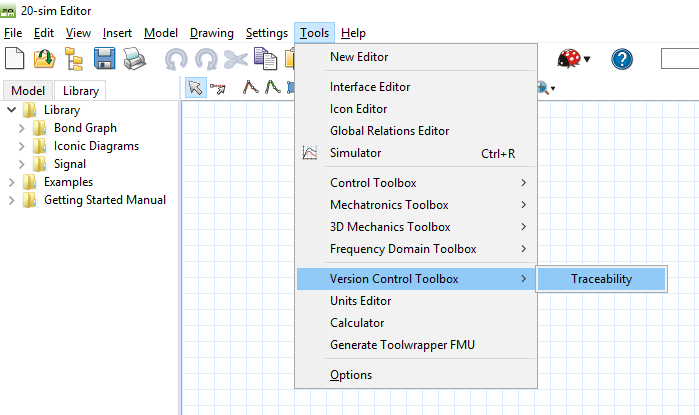
\includegraphics[width=0.7\textwidth]{figures/20sim_TraceabilityDialog1.png}}
	\caption{Opening the traceability dialog in 20-sim.}
	\label{figure:20-sim_traceability_dialog1}
\end{figure}
%
\begin{figure}[ht]
	\centerline{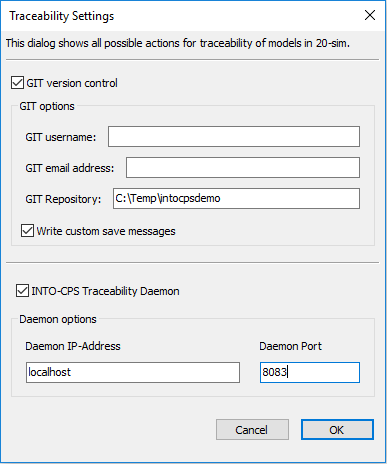
\includegraphics[width=0.6\textwidth]{figures/20sim_TraceabilityDialog2.png}}
	\caption{Opening the traceability dialog in 20-sim.}
	\label{figure:20-sim_traceability_dialog2}
\end{figure}

20-sim has support for several traceable actions:
%
\begin{itemize}
	\item Model creation
	\item Model modification
	\item FMU export
	\item FMU import
	\item Model description XML import
\end{itemize}
%
Performing any of these actions will automatically trigger a trace event. Model creation and model modification are triggered by a \emph{Save As} action and \emph{Save} action respectively in the 20-sim GUI. FMU import and \texttt{model\-Des\-crip\-tion.xml} import are triggered when respectively an FMU or \texttt{model\-Des\-crip\-tion.xml} file is dragged from the Windows Explorer onto the canvas in 20-sim. See also \autoref{sec:simulators:20sim:fmuimport} for more information on how to import an FMU in 20-sim, and \autoref{sec:simulators:20sim:modeldescriptionimport} on how to import a model description XML file into 20-sim. An FMU export event is triggered when an FMU is exported from 20-sim (see \autoref{sec:simulators:20sim:fmuexport} on how to export an FMU from within 20-sim). To read more about what actions are performed during a trace event in 20-sim, please refer to Deliverable D4.3d \cite{INTOCPSD4.3d}.
%
%
%
\subsection{RT Tester}
For Windows, download the latest release bundle of RT-Tester from\\
\url{https://secure.verified.de/f5x1hks4/into-cps/one-click/VSI_bundle.exe}.  Alternatively, you can use the INTO-CPS download manager.  RT-Tester supports tracing the following modelling activities.
%
\begin{itemize}
\item    Define test model
\item    Define test objectives
\item    Run test
\end{itemize}
%
\paragraph{Prerequisites}
Git should be installed in the system, as well as the following Python packages: {\tt requests}, {\tt jsonschema}, {\tt gitpython}.  {\bf Note}: The {\tt VSI\_bundle.exe} installation process this will check whether these are installed; if not, it will be attempted to install them using \texttt{pip}.
%
\paragraph{Configuration of remote OSLC server.}
If the traceability daemon runs on the same system as your RT-Tester, then you
have nothing to configure. The actions will already be identified and traced. 
%
If the daemon is running somewhere else, you can configure this by setting the
environment variable {\tt OSLC\_SERVER}.
%
For example, you can do this from the RTTUI3 as indicated in Figure~\ref{fig:VSI_configure_oscl}:
%
\begin{enumerate}
\item    In the menu bar, select \emph{Project \textrightarrow Project Settings}
\item    Go to the \emph{Local Environment} tab
\item    Click \emph{Add \textrightarrow Add a New Variable}
\item    Set \emph{Name} to {\tt OSLC\_SERVER} and \emph{Value} to the host IP or URL
%
\begin{figure}[htbp]
\centering
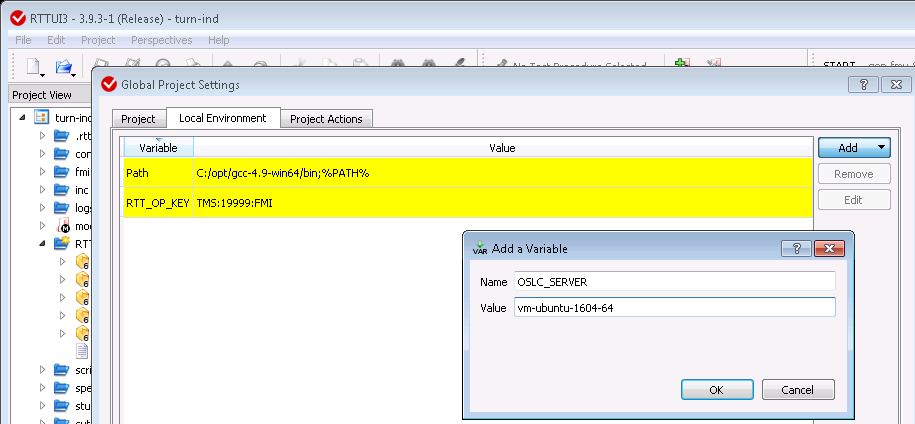
\includegraphics[width=0.99\textwidth]{figures/VSI-rttui3-set-oscl-server}
\caption{Configure variable {\tt OSLC\_SERVER} in RTTUI3.}
\label{fig:VSI_configure_oscl}
\end{figure}
%
\item    Click \emph{OK} to close the \emph{Add Variable} dialog
\item    Click \emph{Save} to close the \emph{Global Project Settings} dialog
\end{enumerate}
%
\subsection{Retrieving Traceability Information}
The following traces can be queried from within the \intoapp:
%
\begin{itemize}
\item FMUs and the related requirements
\item Users and related activities and artifacts
\item Simulation results and the files that were used to produce a certain result
\item Requirements and related test cases
\end{itemize}
%
To get an overview in the Application, right-click on the \emph{Traceability} entry in the project browser and select \emph{Trace Objects}. A page will appear as shown in Figure \ref{fig:trace_overview}.
%
\begin{figure}[htbp]
\centering
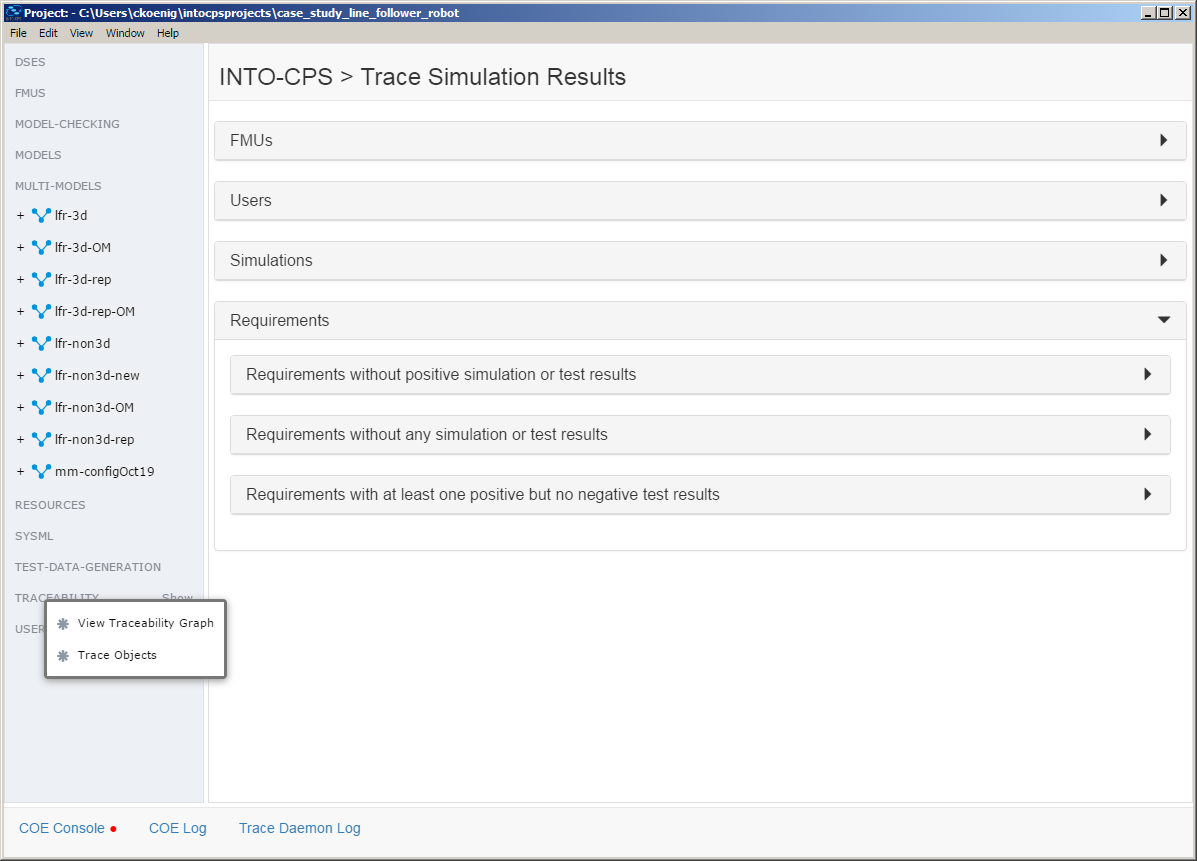
\includegraphics[width=0.99\textwidth]{figures/trace_overview}
\caption{Overview of the different queries as they are implemented in the INTO-CPS Application.}
\label{fig:trace_overview}
\end{figure}
%
\paragraph{Requirements related to FMUs}
In the first tab of the traceability page (\emph{FMUs}) of the INTO-CPS Application (see Figure \ref{fig:trace_overview}), all the FMUs in the traceability database are listed. The FMUs are traced once they are exported from the modelling tool. To each FMU, the related requirements can then be traced, to give the user a quick and easy overview of which requirements are generally linked to a certain FMU, originating from requirements linking in Modelio. 
%
\paragraph{Activities and artifacts related to users}
The second tab (\emph{Users}) lists all the users that have performed traceability-related actions, as identified by their e-mail address. For each user, artifacts (\emph{e.\@g.\@} simulation results, configuration files, \texttt{model\-Des\-crip\-tion.xml} files \emph{etc.\@}) and activities (\emph{e.\@g.\@} exporting an FMU, importing a \texttt{model\-Des\-crip\-tion.xml} file, running a simulation \emph{etc.\@}) can be found, along with the time stamp. This allows evaluating which user created which file, to understand responsibilities in a complex project.
%
\paragraph{Files used to create a simulation result}
The third tab (\emph{Simulations}) lists all the simulation results that were created by the INTO-CPS Application. For each result, the files and the version of the INTO-CPS Application used to create the result can be found. This allows understanding the simulation result and can give confidence, since they can be reconstructed.
%
\paragraph{Test cases and requirements}
The fourth tab (\emph{Requirements}) is sub-divided into three queries. The first, requirements without positive simulation or test results indicates those requirements that have not yet been validated. The second, requirements without any simulation or test result, shows requirements which are not yet covered by a test case, neither positive nor negative. The third, requirements with at least one positive but no negative test result shows those requirements that have had a positive test or simulation result, and can therefore be regarded as fulfilled.